%%%%%%%%%%%%%%%%%%%%%%%%%%%%%%%%%%%%%%
% LaTeX poster template
% Created by Nathaniel Johnston
% August 2009
% Updated by Matthew Denny: May, 2014.
% Further updated to three columns by Sayali Phadke: April 2016
% http://www.nathanieljohnston.com/index.php/2009/08/latex-poster-template/
%%%%%%%%%%%%%%%%%%%%%%%%%%%%%%%%%%%%%%

\documentclass[final]{beamer}
\usepackage{etex}
%\usepackage[size = custom,height = 121.92, width = 99.06,scale=1.1]{beamerposter}
\usepackage[size = custom,height = 99, width = 132,scale=1.1]{beamerposter}
\usepackage{graphicx}	% allows us to import images
\usepackage{natbib}
\usepackage{framed,xcolor}
\colorlet{shadecolor}{black!20}
\usepackage{tabularx}
\usepackage{multirow}
\usepackage[scriptsize]{caption}
\usepackage{amsmath}
\usepackage{amssymb,amsfonts,textcomp}
\usepackage{color,colortbl}
\usepackage{array}
\usepackage{hhline}
\usepackage{tipa}
\usepackage{relsize,exscale}
\usepackage{amsmath}
\usepackage{amssymb}
\usepackage{graphicx}
\usepackage{algcompatible}
%\usepackage{xcolor}
%\usepackage[usenames,dvipsnames]{xcolor}
\definecolor{darkgreen}{RGB}{0,100,0}
\definecolor{verbgray}{gray}{0.9}
\definecolor{maroon}{RGB}{0,23,105}
\definecolor{greyest}{RGB}{90,90,90}
\definecolor{orange}{RGB}{255,127,0}
\definecolor{Grey}{rgb}{0.9,0.9,0.9}
\usepackage[normalem]{ulem}
\newcolumntype{Y}{>{\small\raggedright\arraybackslash}X}
\usepackage{booktabs}
\usepackage[ruled,vlined]{algorithm2e}
\usepackage{dcolumn}
%\usepackage{cite}
%\usepackage{tabular}
\usepackage{multicol}
\usepackage{soul}
\definecolor{lightgray}{gray}{0.85}
\sethlcolor{lightgray}


\newtheorem{hypothesis}{Hypothesis}
\definecolor{umassblue}{HTML}{333399}
\definecolor{umassred}{HTML}{001769}
\definecolor{darkblue}{rgb}{0.5,0.3,0.7}

% Alternate bibliography styles
% \usepackage{natbib}
% \bibliographystyle{apalike}

% Hyper Reference Formatting
\usepackage{hyperref}
\hypersetup{colorlinks,breaklinks,
            linkcolor=darkblue,urlcolor=darkblue,
            anchorcolor=darkblue,citecolor=darkblue}



%\bibliographystyle{$HOME/Documents/bibtex.utils/jss}
\usepackage{hyperref}
%-----------------------------------------------------------
% Define the column width and poster size
% To set effective sepwid, onecolwid and twocolwid values, first choose how many columns you want and how much separation you want between columns
% The separation I chose is 0.024 and I want 4 columns
% Then set onecolwid to be (1-(4+1)*0.024)/4 = 0.22
% Set twocolwid to be 2*onecolwid + sepwid = 0.464
%-----------------------------------------------------------
%-----------------------------------------------------------
% Define the column width and poster size
% To set effective sepwid, onecolwid and twocolwid values, first choose how many columns you want and how much separation you want between columns
% I keep the separation as 0.025 and I want 3 columns
% Then set onecolwid to be (1-(3+1)*0.025)/3 = 0.3
% Set twocolwid to be 2*onecolwid + sepwid = 0.625
%-----------------------------------------------------------

\newlength{\sepwid}
\newlength{\onecolwid}
\newlength{\onecolwidd}
\newlength{\twocolwid}
%\newlength{\threecolwid}
\setlength{\paperwidth}{30in}
\setlength{\paperheight}{40in}
\setlength{\sepwid}{0 \paperwidth}
\setlength{\onecolwid}{0.35\paperwidth}
\setlength{\onecolwidd}{0.54\paperwidth}
\setlength{\twocolwid}{0.675\paperwidth}
%\setlength{\threecolwid}{0.675\paperwidth}
\setlength{\topmargin}{1in}
\usetheme{confpostervert}
\setlength{\leftmargin}{1in}% 
\setlength{\rightmargin}{0in}% 

%-----------------------------------------------------------
% Define colours (see beamerthemeconfposter.sty to change these colour definitions)
%-----------------------------------------------------------

\setbeamercolor{block title}{fg=umassred,bg=white}
\setbeamercolor{block body}{fg=black,bg=white}
\setbeamercolor{block alerted title}{fg=white,bg=umassred!70}
\setbeamercolor{block alerted body}{fg=black,bg=umassred!10}




\setbeamersize{text margin left=0cm,text margin right=0cm}
%\newlength\MyColSep
%\setlength\MyColSep{1cm}
%\newlength\MyColWd
%\setlength\MyColWd{0.22\textwidth -0.66666\MyColSep}






%-----------------------------------------------------------
% Name and authors of poster/paper/research
%-----------------------------------------------------------

\title{Testing for Network Effects in Field Experiments: Examples from Legislative Studies}
\author{Sayali Phadke$^{\dag 1}$, Bruce A. Desmarais$^{\dag 2}$}
\institute{$^\dag$Pennsylvania State University; | \texttt{$^1$sayalip@psu.edu; $^3$bdesmarais@psu.edu}}

%-----------------------------------------------------------
% Start the poster itself
%-----------------------------------------------------------
% The \rmfamily command is used frequently throughout the poster to force a serif font to be used for the body text
% Serif font is better for small text, sans-serif font is better for headers (for readability reasons)
%-----------------------------------------------------------

\begin{document}

\begin{frame}[t]

	\begin{columns}[t]	% the [t] option aligns the column's content at the top

	%first column	
	\begin{column}{\onecolwidd}
			
		
		\begin{alertblock}{Research Objectives}
				\begin{rmfamily}
					\begin{large}
%						\vskip0.5ex
						
						\begin{itemize}
							\item Model spillover of treatment effect via network structures. 
							\vspace*{.1in}
							\item Examine how inferences depend upon the specification of the network and spillover structure.
							\vspace*{.1in}
							\item Evaluate the models using data from field experiments on US State legislatures. 
							
					
						\end{itemize}
						
						\vskip0.5ex
					\end{large}
				\end{rmfamily}
			\end{alertblock}
	%These work like sections, use them to break up the content -- note that they do not span columns		
	\vspace{.2in}
	\begin{block}{Motivation}
	\begin{rmfamily}
	\begin{itemize}
	
	\item Conventional causal inference methods rely on SUTVA (Stable Unit Treatment Value Unit Assumption)
	\vspace*{.1in}
		\begin{itemize}
		\item SUTVA assumes that the outcome of a unit is unaffected by the treatment statuses of other units
		\end{itemize}
		\vspace*{.1in}	
	\item However, most social processes involve complex interaction and dependence among networked units
	\vspace*{.1in}
	\item Interpersonal interactions propagate treatment effect to control units and
	\vspace*{.1in}
	\item Various factors impact how and how much the treatment effect spreads
	\vspace*{.1in}
	\item Must account for the interference structure to correctly estimate the treatment effect
	\vspace*{.1in}
	\item Understanding the propagation of treatment itself of interest in policy planning or marketing strategy
	
	\end{itemize}


	\vspace*{.3in}	
\centering
\begin{figure}
\centering
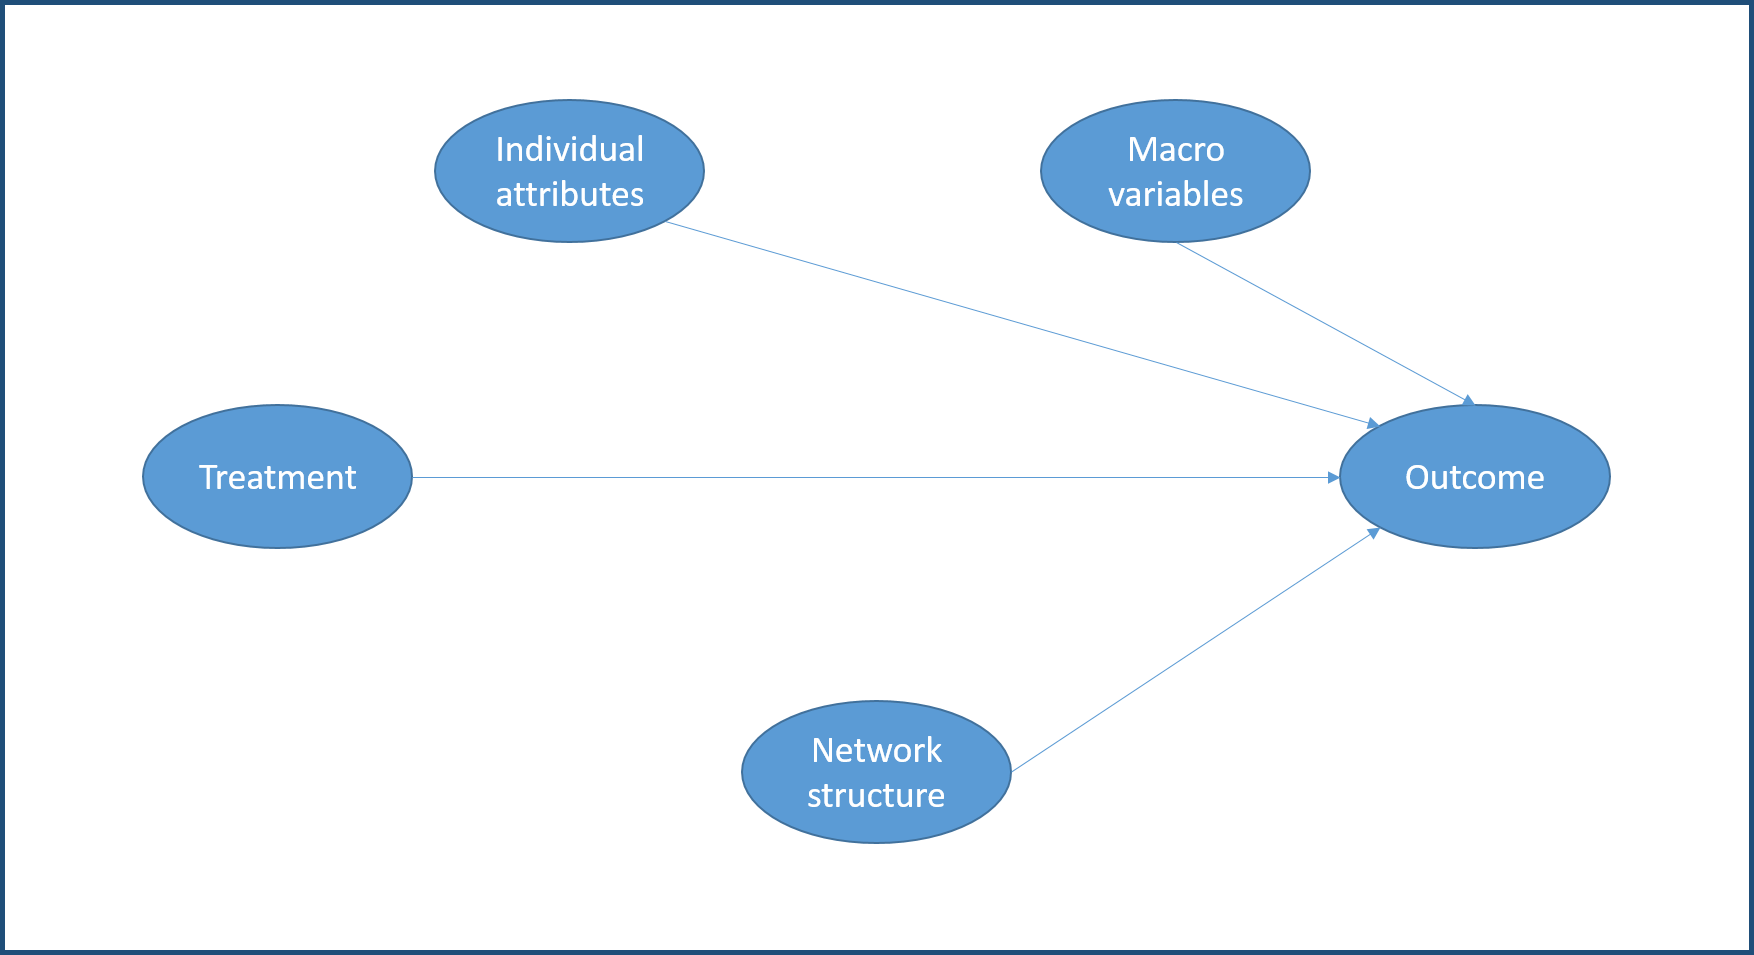
\includegraphics[scale=0.8]{Individual_structure.png}
\vspace*{5mm}
\caption{\small \textbf{Individual causal diagram}: In addition to the unit's treatment status, the network structure and treatment assignments within it are also important in determining its outcome}
\end{figure}
\vspace*{-10mm}
\centering
\begin{figure}
\centering
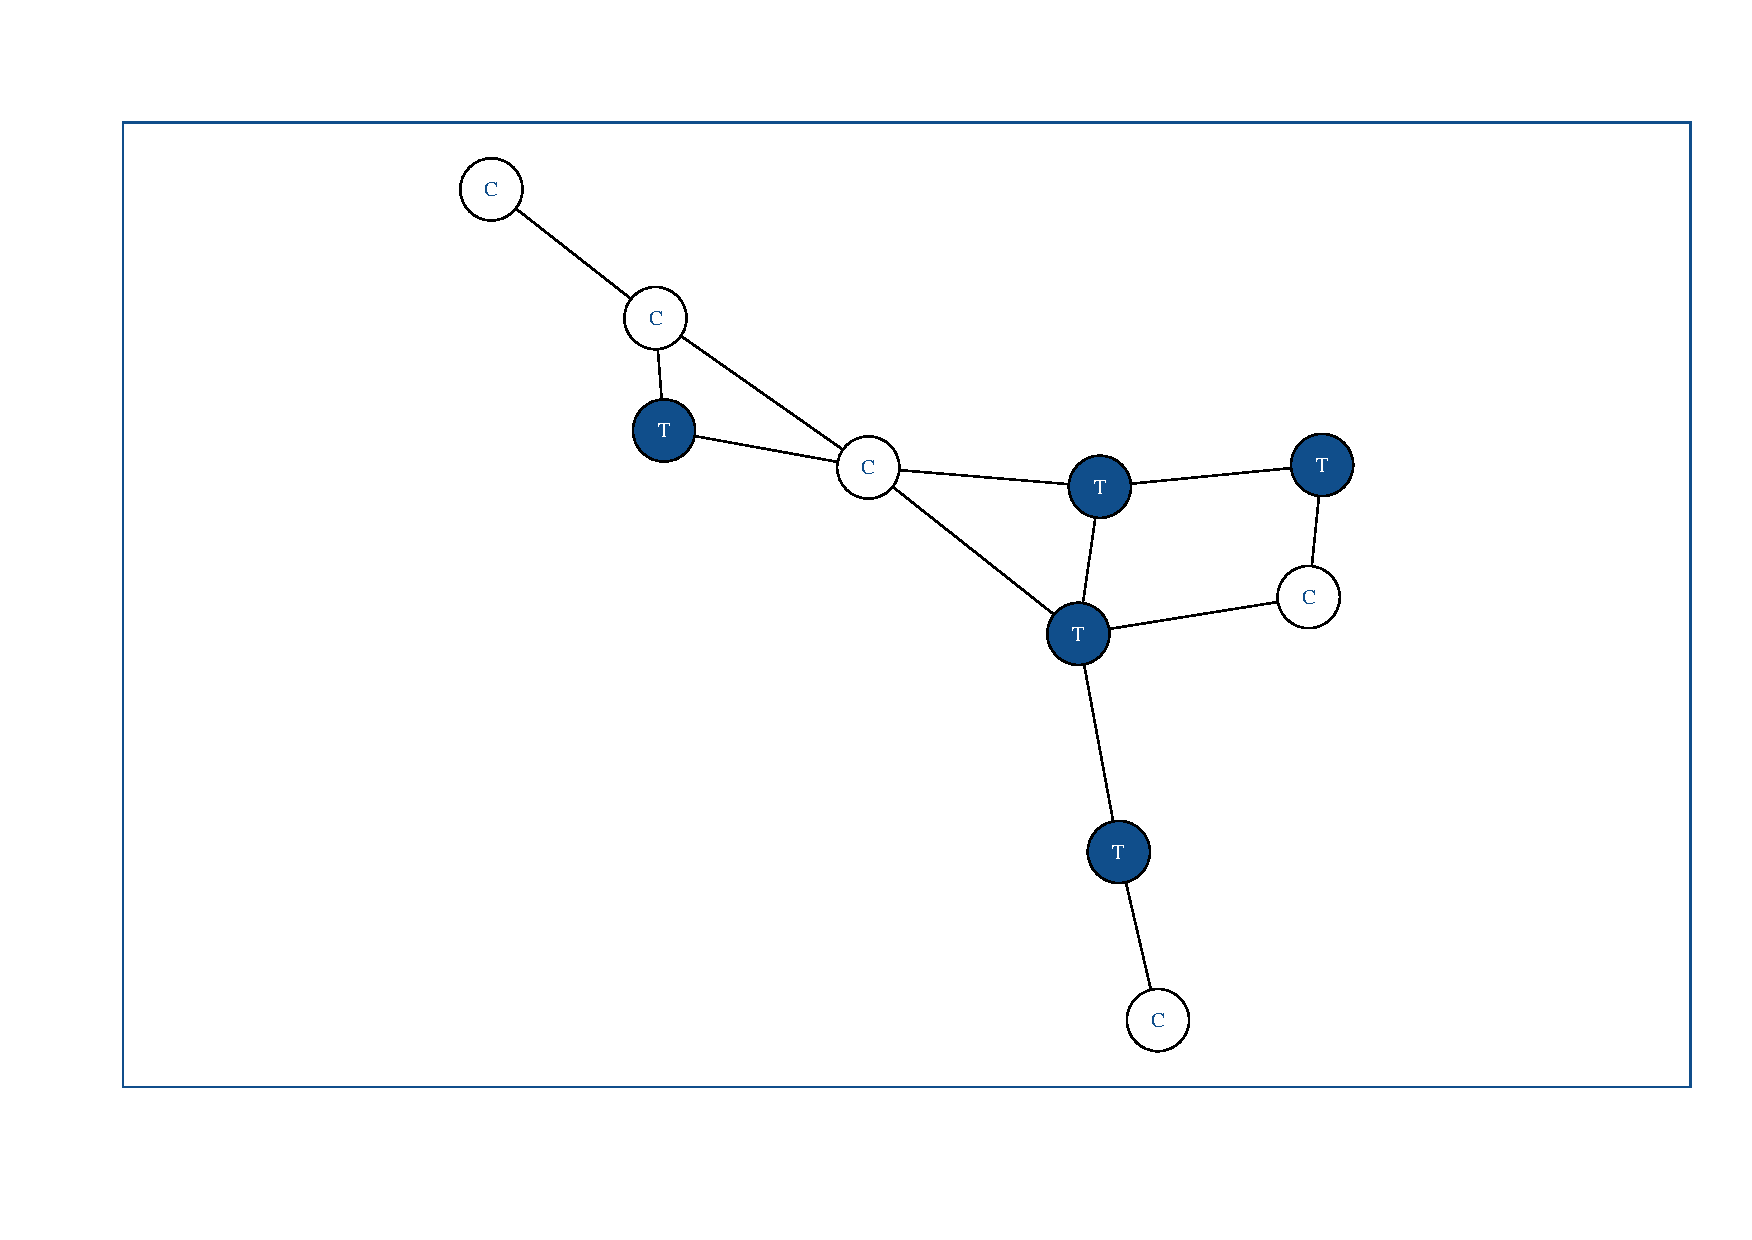
\includegraphics[scale=0.8]{Dummy_network.pdf}
\vspace*{-15mm}
\caption{\small \textbf{Network plot: How would we expect the treatment to affect untreated units?} Simple illustration showing possible neighborhoods of control units. \textbf{T: treated unit and C: control}}
\end{figure}	
	
	\end{rmfamily}
	\end{block}
	
	\begin{block}{Existing Approaches}
		\begin{rmfamily}
	
	{\large \textbf{Bowers et. al. method:}}\\
	\citealt{bowers2012reasoning} proposed a non-parametric testing method for interference effects. Overall idea of this method is as follows:

	\begin{itemize}
	\item Assume the "sharp null hypothesis of no effects" i.e. treatment assignment has no effect on any unit
	\vspace*{.1in}
	\item Specify causal model describing the change in potential outcomes when treatment assignment changes
	\vspace*{.1in}
	\item  Map potential outcomes from the causal model to observed outcomes
	\vspace*{.1in}
	\item Assume treatment only spreads along edges and spillover depends on the number of treated neighbors
	\vspace*{.1in}	
	\item Test statistic should be a small value when distribution of treated and control outcomes in the adjusted data are similar, and a large value when distributions are dissimilar
	\vspace*{.1in}
	\item p-value is the proportion of permutation tests whose test statistic is lesser than the observed test statistic
	\vspace*{.1in}	
	\end{itemize}
	\end{rmfamily}
	\end{block}
	

\end{column}		
	\begin{column}{\onecolwidd}
	
	\begin{block}{Existing Approaches}
		\begin{rmfamily}
	
	{\large \textbf{Coppock application}}\\
	\citealt{coppock2014information} implements Bowers method to analyze the New Mexico Legislator experiment conducted by \citealt{butler2011can}. Uses ideological network with a different choice of diffusion model and test statistic. Bowers methodology is inadequate to handle categorical outcomes.
	
	\end{rmfamily}
	\end{block}
	
	\hspace{2cm}
						
	\vspace*{10mm}
	\begin{block}{Proposed extensions along salient dimensions}
	\begin{rmfamily}
	
	\begin{itemize}
	
	\item \textbf{Neighborhood specification:}
		\begin{multicols}{2}
		\begin{itemize}
		\item Effect from all units
		\item Effect from k-nearest neighbors 
		\end{itemize}
		\end{multicols}
		\vspace*{.02in}
	\item \textbf{Diffusion model specification:} Consider models varying along following dimensions:
		\begin{multicols}{2}
		\begin{itemize}
		\item Distance from the nearest treated node
		\item Number/proportion of treated neighbors
		\item Form of spread (linear or non-linear)
		\end{itemize}
		\end{multicols}
		\vspace*{.02in}
	\item \textbf{Network selection:}
		\begin{multicols}{2}
		\begin{itemize}
		\item Ideological network
		\item Committee network
		\item Co-sponsorship network
		\item Geographical network network
		\end{itemize}
		\end{multicols}
		\vspace*{.02in}	
	\item \textbf{Test statistic selection:}
		\begin{multicols}{2}
		\begin{itemize}
		\item Kolmogorov-Smirnov test
		\item Anderson-Darling test
		\item Mann-Whitney U test
		\item Control Median test
		\end{itemize}
		\end{multicols}
		\vspace*{.02in}
	\end{itemize}	

	\end{rmfamily}						
	\end{block}
	
	\vspace*{10mm}
	\begin{block}{Data}
	\begin{rmfamily}
	
	Bill to return a projected budget surplus in form of a rebate proposed in the New Mexico state legislature during a special session in 2008. 35 out of the 70 legislators (matched pairs) received estimates of support within their constituencies. Below are three possible network structures connecting the legislators:
	
	\hspace{2cm}
	\begin{figure}
	\centering
	\begin{tabular}{ccc}
	{\bf Ideological Network (top 5\%)} & {\bf Geographic Network} & {\bf Committee Network (>1 common)}\\
	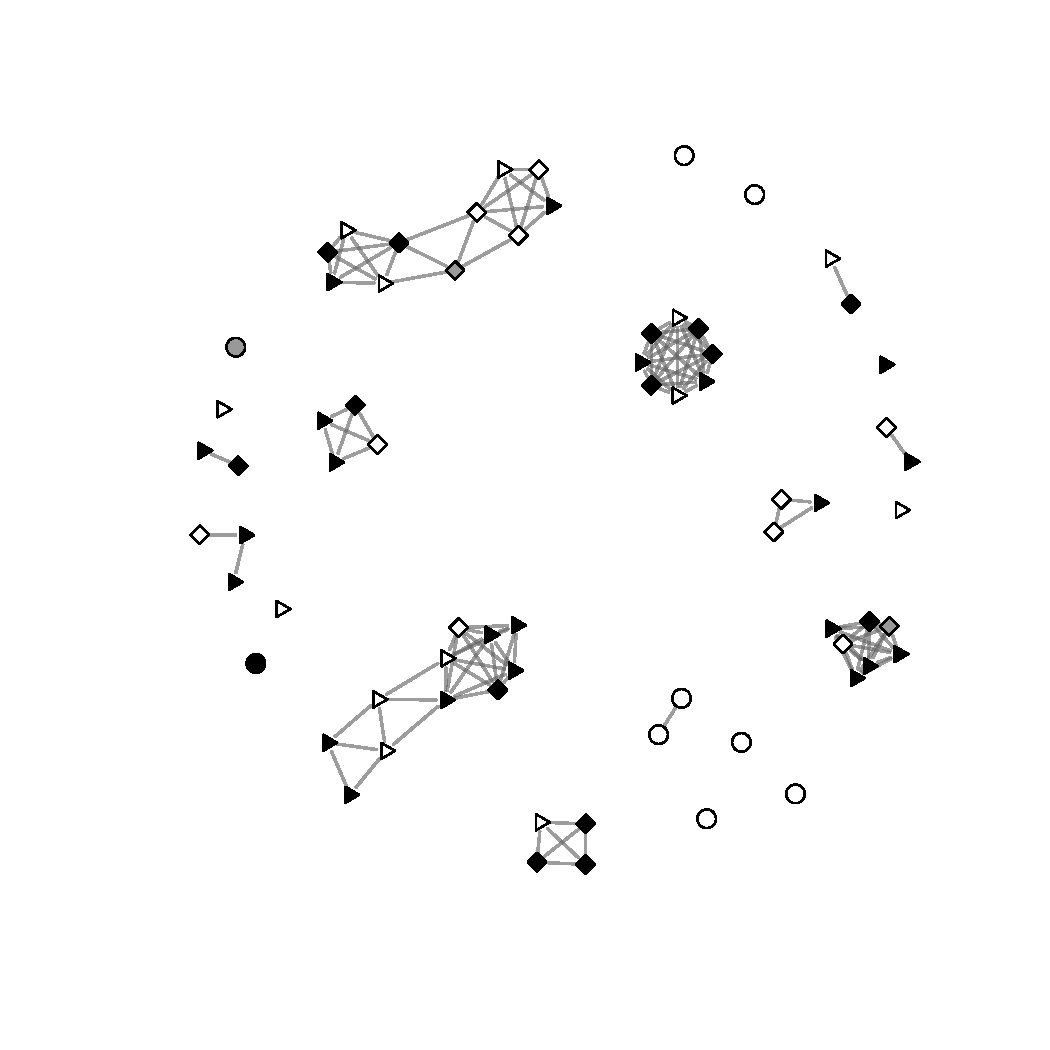
\includegraphics[scale=0.8, clip=true,trim =2cm 2cm 2cm 2cm]{coppock_ideological_net.pdf} &
	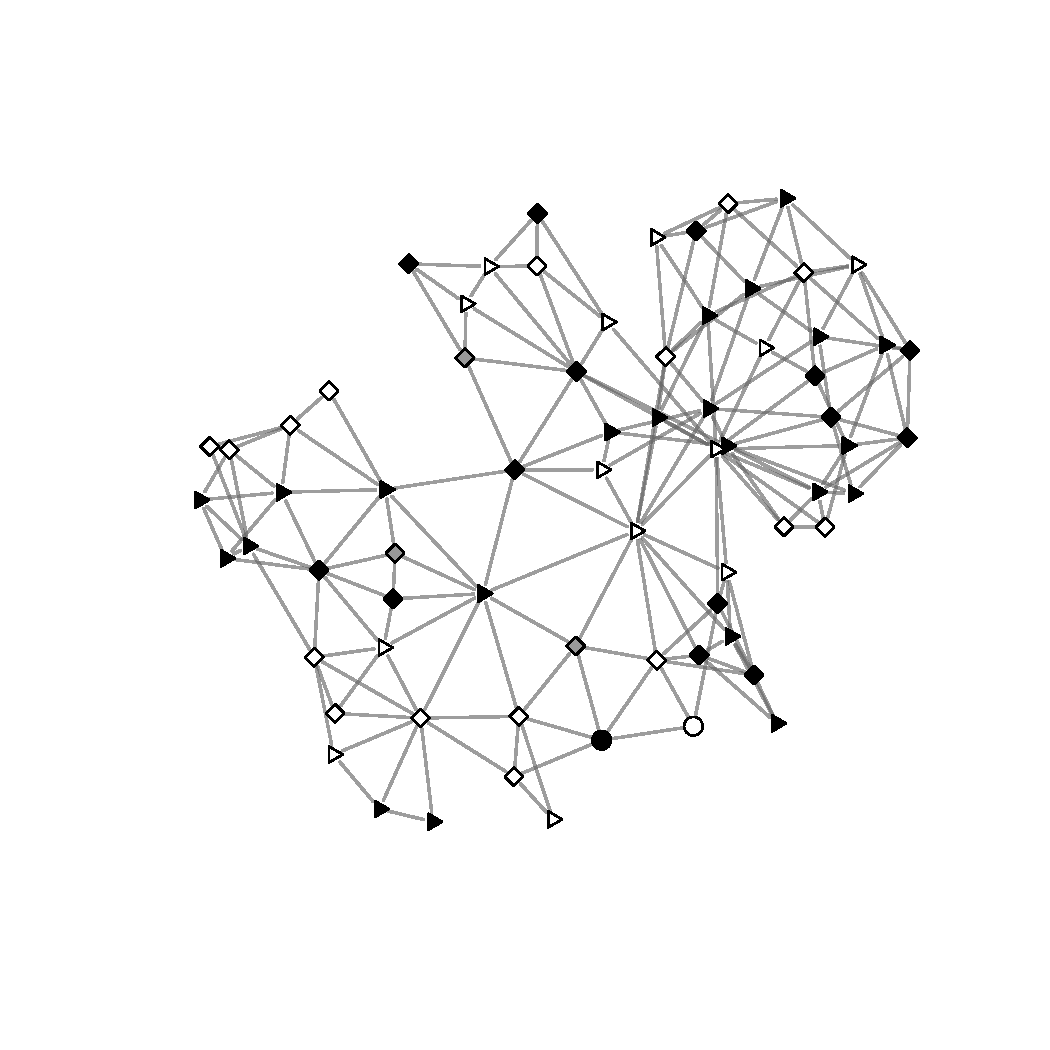
\includegraphics[scale=0.8, clip=true,trim =2cm 2cm 2cm 2cm ]{coppock_geographic_net.pdf} & 
	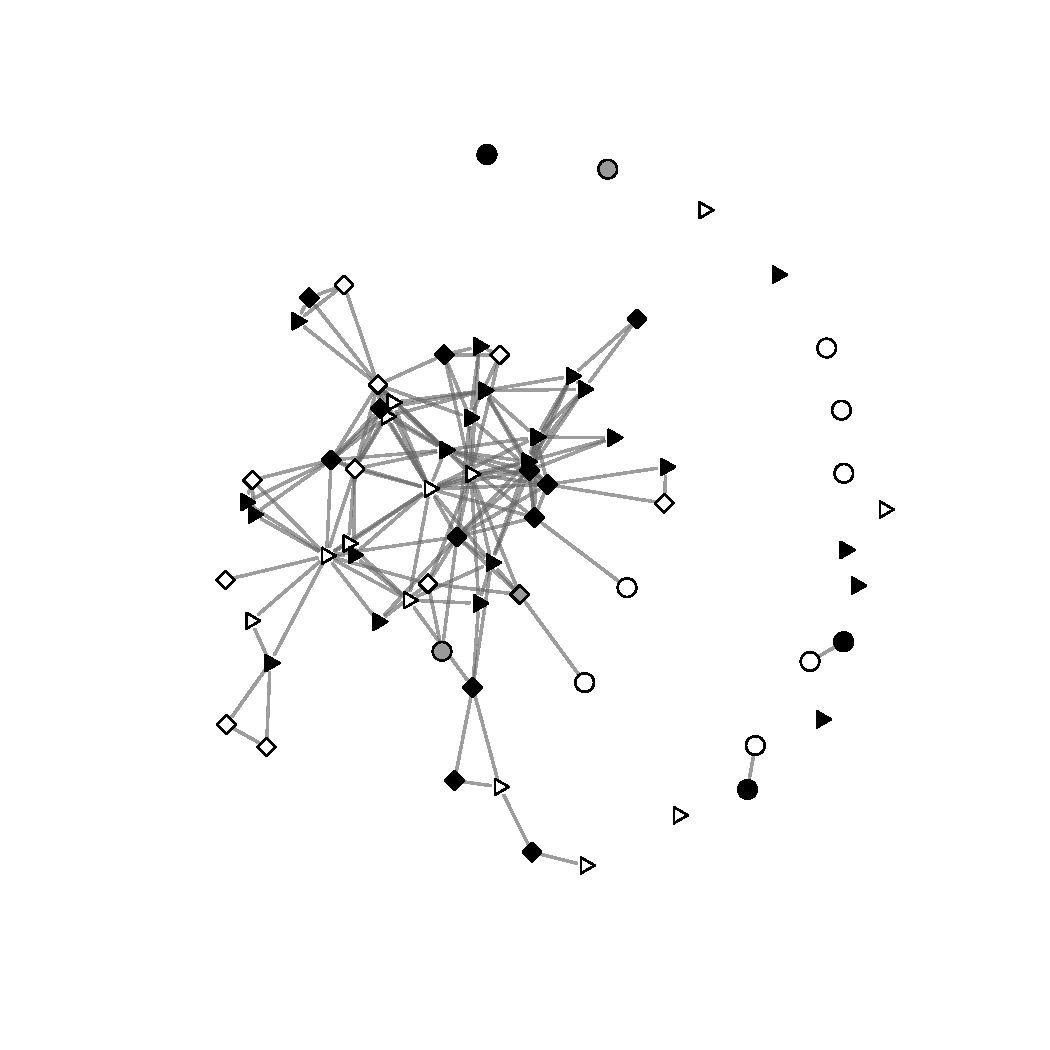
\includegraphics[scale=0.8, clip=true,trim =2cm 2cm 2cm 2cm]{nm_committee_net.pdf} \\ 
	\end{tabular}
	\vspace*{10mm}
	\caption{Different networks among New Mexico legislators. Colors denote outcome: black means voted with district, gray means abstained, white means voted against. Shape denotes treatment status. Triangles are treated. Squares are adjacent to treated. Circles are isolated from treatment}
	\label{fig:nh-nets}
	\end{figure}

	\end{rmfamily}						
	\end{block}
	
	\begin{block}{Replication of Coppock analysis}
	\begin{rmfamily}
	
	\vspace{-8mm}
	\begin{figure}
	\centering
	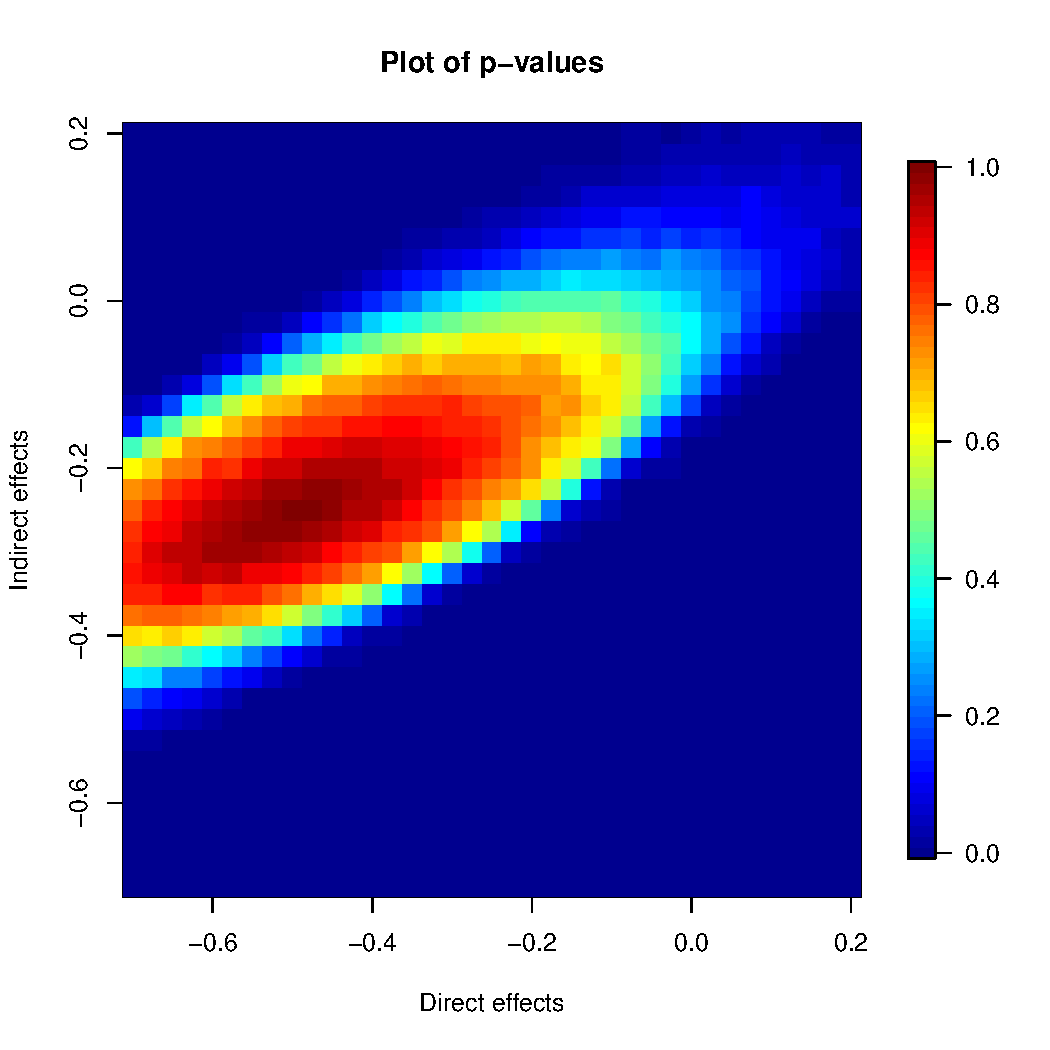
\includegraphics[scale=0.7]{pvalues_figure.pdf}
	\caption{\textbf{Higher values provide evidence for spillover effect}}
	\end{figure}

	\end{rmfamily}						
	\end{block}

	
	\end{column}



\begin{column}{\onecolwidd}

	\begin{block}{Extension}
	\begin{rmfamily}
	
	\textbf{Neighborhood specification:}
	Extend the Coppock analysis using ideological scores and creating an adjacency matrix based on whether a particular legislator is one of the k nearest neighbors
	
	\hspace{2cm}
	\begin{figure}
	\centering
	\begin{tabular}{cc}
	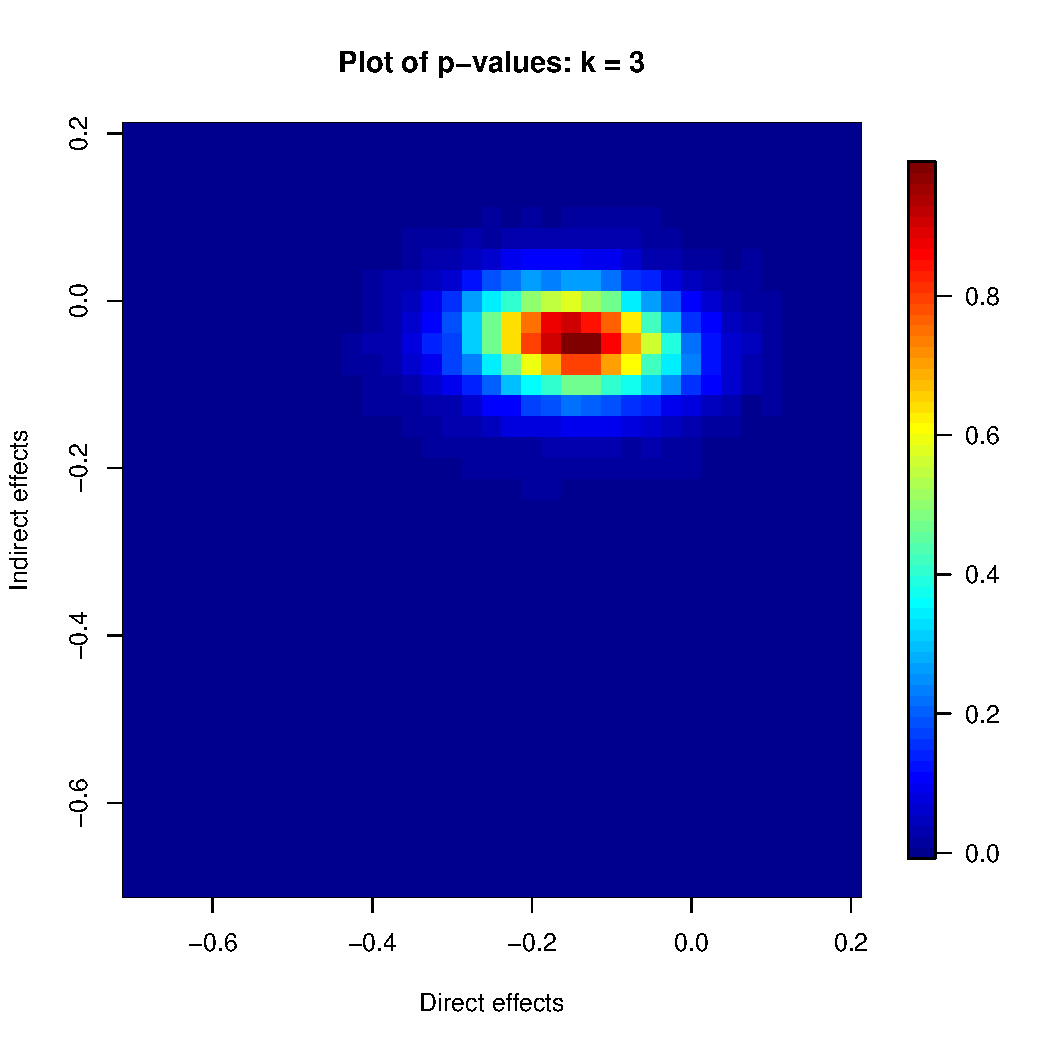
\includegraphics[scale=0.7]{pvalues_figure_3nn.pdf} &
	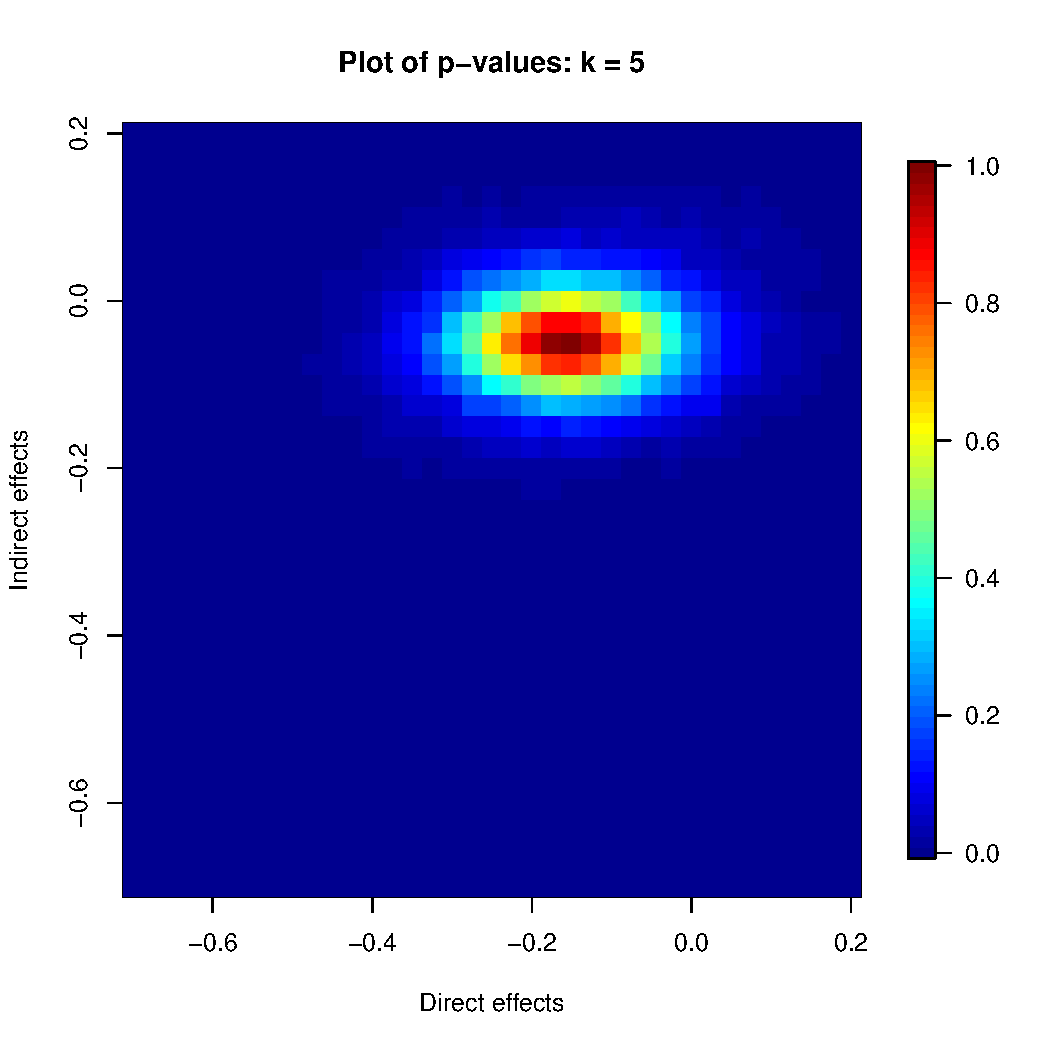
\includegraphics[scale=0.7]{pvalues_figure_5nn.pdf} \\ 
	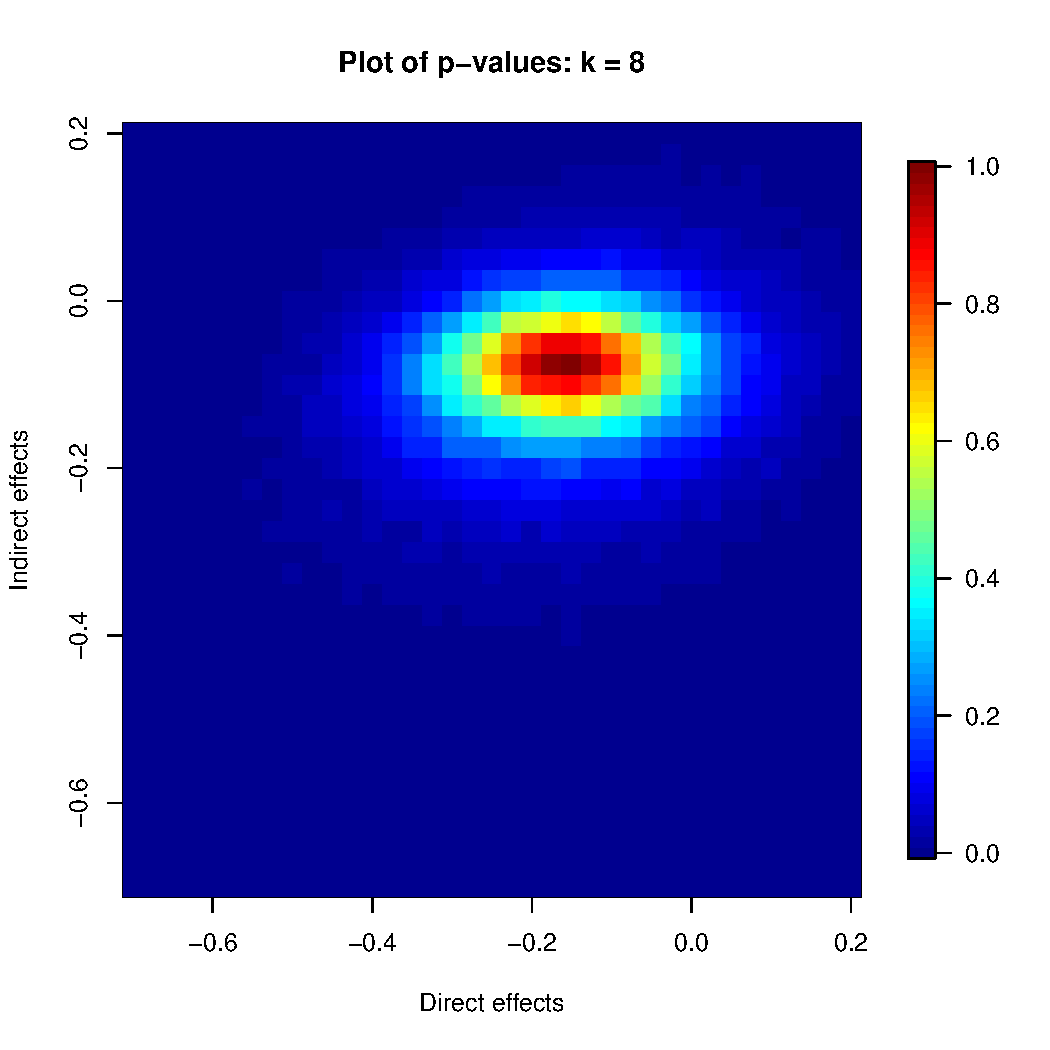
\includegraphics[scale=0.7]{pvalues_figure_8nn.pdf} &
	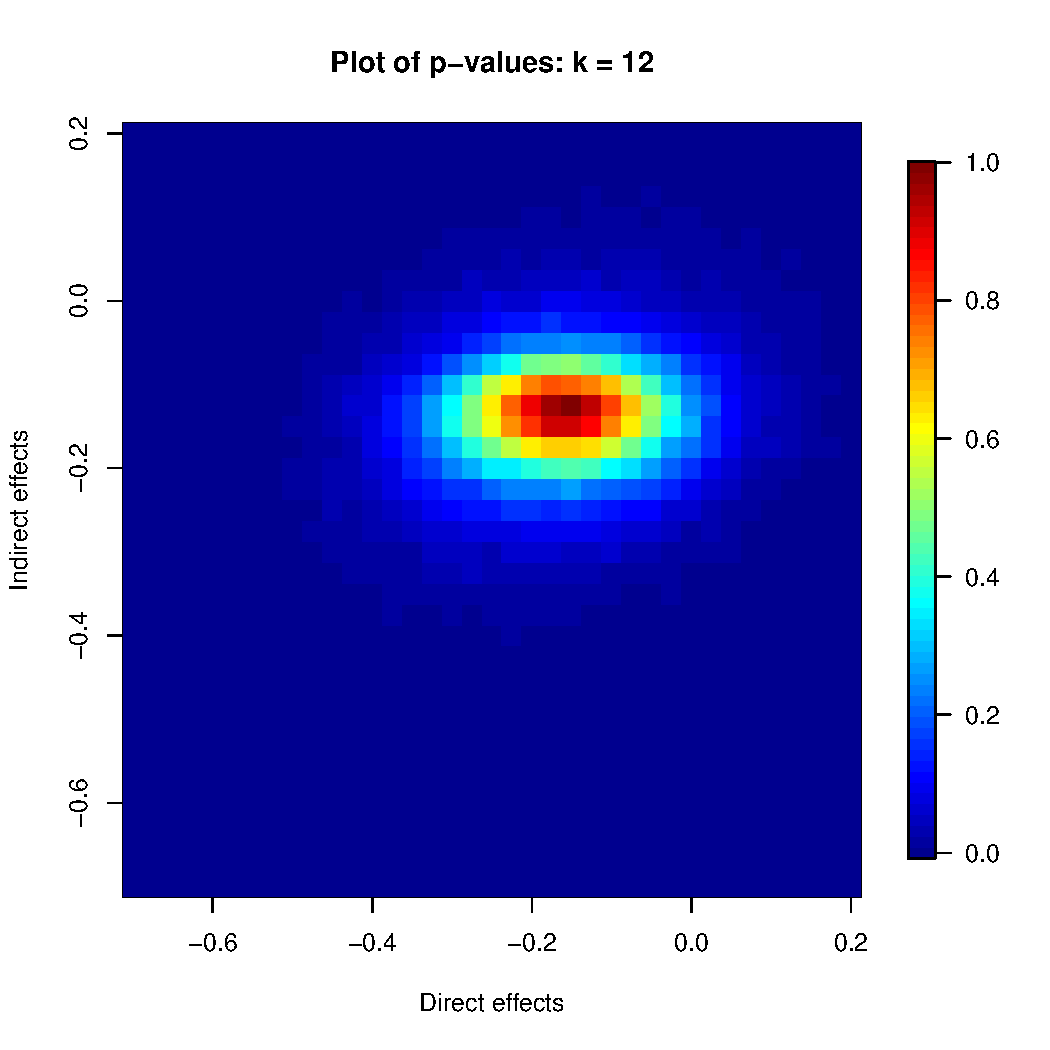
\includegraphics[scale=0.7]{pvalues_figure_12nn.pdf} \\ 
	\end{tabular}
	\caption{p-values: highest values move closer to zero value for both effects}
	\end{figure}
	
	\textbf{Network selection:}
	Extend the Coppock analysis using committee network. Undirected tie exists between legislators who have served on two or more legislative committees together
	
	\hspace{2cm}
	\begin{figure}
	\centering
	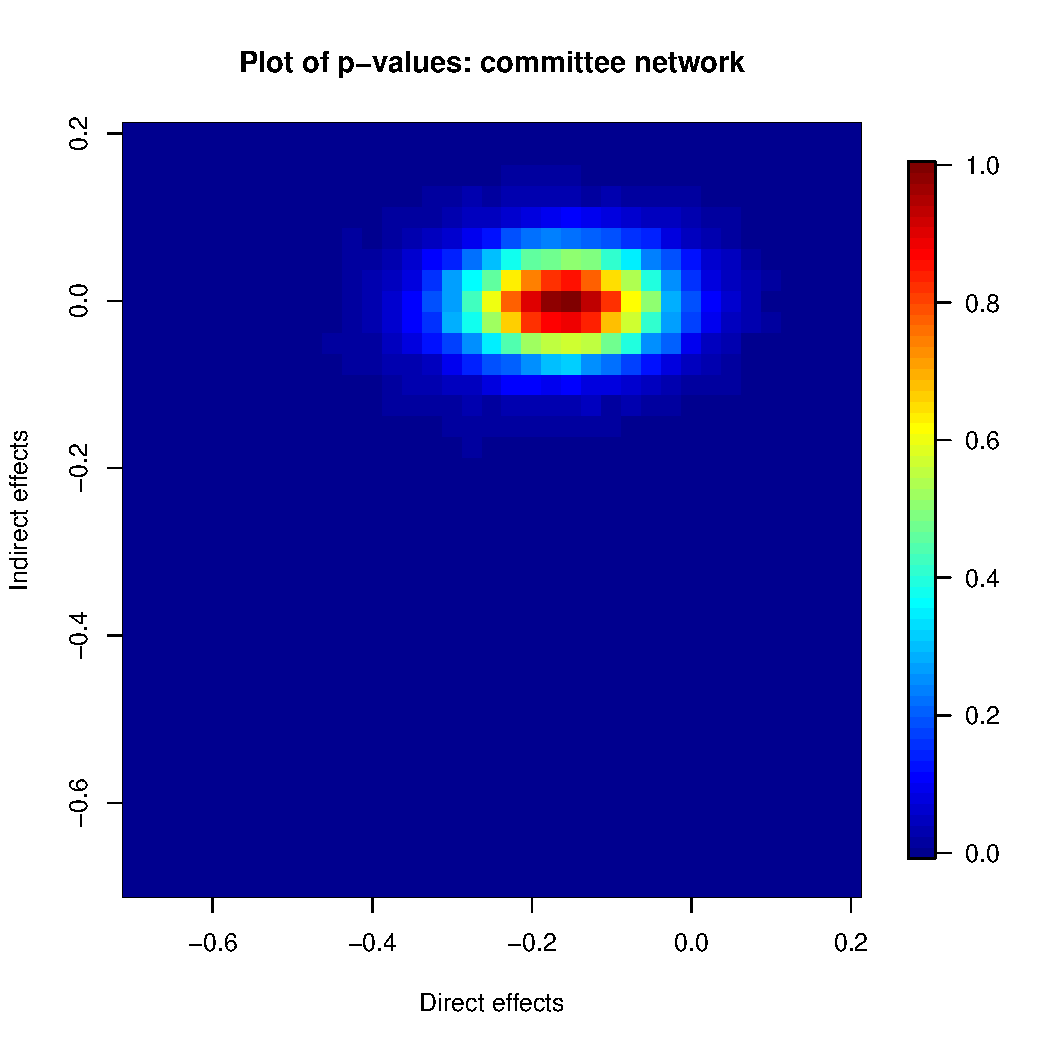
\includegraphics[scale=0.7]{pvalues_figure_committee.pdf}
	\caption{p-values: does not show evidence of network effect}
	\end{figure}
			
	\end{rmfamily}						
	\end{block}
	
	\vspace*{10mm}
	\begin{block}{Future direction}
	\begin{rmfamily}
	
	\begin{itemize}
	\item Consider another example of a field experiment on New Hampshire state legislature
	\vspace*{.1in}
	\item Evaluate models specified by various dimensions under the extensions
	\vspace*{.1in}
	\end{itemize}
		
	\end{rmfamily}						
	\end{block}
	
	\vspace*{10mm}

	\begin{block}{References}
	\begin{rmfamily}
	\bibliographystyle{apsr}
	\bibliography{poster}
	\end{rmfamily}
	\end{block}

	\end{column}	
	\end{columns}
	
	
%%%% Footnotes part

	\vspace{.9in} % adjust to put footer in correct place		
	\hspace*{.025in} \begin{beamercolorbox}[wd=50.75in,colsep=0.1cm]{cboxb}\end{beamercolorbox}
	\vspace{0.25in}
			
	\begin{columns}
		\vspace{0.3in}
		\begin{column}{0.3\paperwidth}	
				\centering
		\begin{tabular}{cc}

 \begin{minipage}{8.5in}
 \begin{rmfamily}
This material is based on work supported by the National Science Foundation under IGERT Grant DGE-1144860, Big Data Social Science.
\end{rmfamily}

\end{minipage}

& 
\begin{minipage}{2.5in}
%\bigskip
\includegraphics[scale=.25]{NSF_logo.png}
\end{minipage}
\end{tabular}
	
		\end{column}
		
		
		\begin{column}{0.3\paperwidth}
		\end{column}
		
		\begin{column}{0.3\paperwidth}

	\begin{center}
	\begin{figure}
	\centering
	\begin{tabular}{cc}
	
\includegraphics[scale=0.64]{BDSS_logo.jpg} &
	
\includegraphics[scale=0.123]{PSU_logo_2.jpg} \\ 
	\end{tabular}
	\end{figure}
	\end{center}
			
		\end{column}

		\vspace{1cm}	
	\end{columns}
	
	
	

\end{frame}

\end{document}
